% 
% 

\begin{frame}{$\nu$ mass \& mixing: Only known window to new physics}

That new physics is not well understood:\\
\vspace{0.2cm}
%\begin{itemize}
%\item Discovery of neutrino masses and mixings: {\color{red} \bf BSM physics}!
%\item New physics not understood
{
\begin{itemize}
  \item {\bf What is the mass generation mechanism?}
  {
    \begin{itemize}
       \item Could the neutrino be a Majorana particle?
       \item Why are the masses so small?
    \end{itemize}
  }
  \item {\bf Does it explain flavour?}
  {
    \begin{itemize}
       \item Nearly (exactly?) maximal mixing observed: `$\mu$' and `$\tau$' flavour interchangeable in neutrino oscillations.
    \end{itemize}
  }
  \item {\bf Does it provide a connection between the quark and lepton sectors?}
  {
    \begin{itemize}
       \item Why the corresponding mixing matrices are so different?
    \end{itemize}
  }
  \item {\bf What are the implications for the universe we live in?}
  {
    \begin{itemize}
       \item Baryon asymmetry of the universe: CP violation + Majorana masses ingredients of the leptogenesis hypothesis.
       \item Dark matter: Sterile neutrino is a candidate.
    \end{itemize}
  }
\end{itemize}
}
%\end{itemize}
%\begin{block}{}
%{\scriptsize \bf
%\begin{center}
%{\color{magenta}The study of neutrino masses and mixings the only known window to new physics.}
%\end{center}
%}
%\end{block}
\end{frame}




\begin{frame}{Two squared-mass splitting scales}

\begin{columns}
  \begin{column}{0.50\textwidth}
    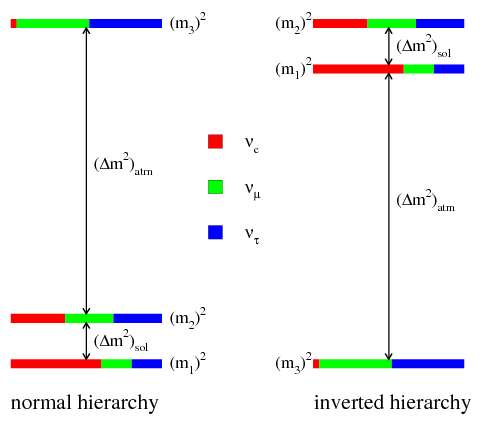
\includegraphics[width=0.95\textwidth]{./images/etc/mh.png}
  \end{column}
  \begin{column}{0.50\textwidth}
    As you have seen at the previous lectures, we have now observed oscillations at both squared-mass splitting scales\\
    \vspace{0.2cm}
    \begin{itemize}
      \item {\color{red} \bf the "solar" splitting}\\
             \vspace{0.2cm}
            {\bf ${\Delta}m^{2}_{21}$ }   $\approx$ 7.5 $\times 10^{-5}$ $eV^{2}/c^{4}$\\
      \vspace{0.3cm}
      \item {\color{red} \bf the "atmospheric" splitting}\\
             \vspace{0.2cm}
            {\bf $|{\Delta}m^{2}_{32}|$ } $\approx$ 2.5 $\times 10^{-3}$ $eV^{2}/c^{4}$\\
    \end{itemize}   
  \end{column}
\end{columns}

\end{frame}

